%! Author = Len Washington III
%! Date = 8/12/2023

% Preamble
\documentclass[3]{cs430homework}

% Document
\begin{document}

\maketitle

\begin{enumerate}[label=\arabic*.]
	\item (10 points) Given a set of $n$ numbers, we wish to find the $i$ largest numbers in sorted order utilizing the comparison-based algorithm/data structure specified. Each algorithm should return an array of the $i$ largest numbers in sorted order, lowest to highest. \emph{For each of your algorithms, find a theta bound on the worst-case running time in terms of $n$ and $i$.}
	\begin{enumerate}[label=\arabic{enumi}\alph*)]
	    \item Write an algorithm to find the $i$ largest numbers in sorted order using a max heap.
		\item Write an algorithm to find the $i$ largest numbers in sorted order using the $i$th largest order-statistic algorithm.
	\end{enumerate}
	\item (4 points) Give an $O(n)$ algorithm for the following problem and prove its time complexity. Given a list of $n$ distinct positive integers, partition the list into two sublists, each of size $n/2$, such that the difference between the sums of the integers in the two sublists is maximized. You may assume that $n$ is a multiple of 2.
	\item (4 points) Suppose we use RANDOMIZED-SELECT to select the minimum element of the array $A=<3,2,9,0,7,5,4,8,6,1>$. Describe a sequence of partitions that results in a worst-case performance of RANDOMIZED-SELECT.
	\item (6 points) Argue that since sorting $n$ elements takes $\Omega(n \lg n)$ time in the worst case in the comparison model, any comparison-based algorithm for constructing a binary search tree from an arbitrary list of $n$ elements must take $\Omega(n \lg n)$ time in the worst case. Basically, prove you cannot construct a BST in linear growth time. Hint: To sort with a binary search tree you must first construct the binary search tree and then traverse the binary search tree in such a way so the output is sorted.
	\item (6 points)\\
\begin{minipage}{0.6\textwidth}
The set of full binary trees is defined recursively: Basis step: The tree consisting of a single vertex is a full binary tree.\\

Recursive step: If $T1$ and $T2$ are disjoint full binary trees, there is a full binary tree, denoted by $T1 \times T2$, consisting of a root $r$ together with edges connecting $r$ to each of the roots of the left subtree $T1$ and the right subtree $T2$.\\

Use structural induction to show that $l(T)$, the number of leaves of a full binary tree $T$, is 1 more than $i(T)$, the number of internal vertices of $T$.
\end{minipage}\hfill
\begin{minipage}{0.35\textwidth}
	 \begin{figure}[H]
		 \centering
		 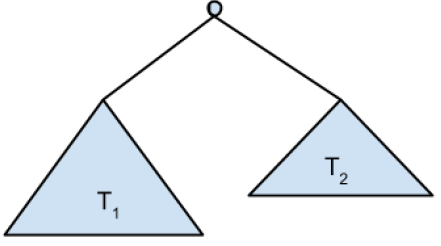
\includegraphics[width=\textwidth]{3.5}
		 \caption{}
		 \label{fig:3.5}
	 \end{figure}
\end{minipage}
	\item (5 points) Is the operation of deletion ``commutative'' in the sense that deleting $x$ and then $y$ from a binary search tree leaves the same tree as deleting $y$ and then $x$? Argue why it is or give a counterexample.
	\item (5 points)
	\begin{enumerate}[label=\arabic{enumi}\alph*)]
	    \item How many different binary search trees are there for values $1$ $2$ $3$?
		\item How many different orders are there for inserting the values $1$ $2$ $3$ in a binary search tree?
		\item Are these values the same? Why or why not?
	\end{enumerate}
\end{enumerate}

\end{document}